\subsection{Model 1: Salience Biased Affinity Propagation Clustering}

  \begin{figure}
\begin{algorithmic}[1] 
\Procedure{APSalienceSummarize}{}
  \State $\updates \gets \varnothing$ \Comment{Init. update summary.}
  \For{$\strsents_t \in \strsents$} 
    \State $\hat{\Salience} \gets \operatorname{salience}(\strsents_t, \query)$
        \Comment{Estimate sentence salience for each 
                 $\strsent \in \strsents_t$.}
    \State $\Similarity \gets \operatorname{similarity}(
           \strsents_t, \strsents_t)$ \Comment{Compute similarity 
           between each $\strsent_i, \strsent_j \in \strsents_t$.}
    \State $\exemplars \gets \operatorname{AffinityPropagation}(\hat{\Salience}, \Similarity)$ \Comment{Get exemplar sentences $\exemplars$ with AP.}

    \For{$\strsent \in \exemplars$}
      \If{$\hat{\Salience}_\strsent > \lambda_1 \wedge \max \operatorname{similarity}(\updates, \strsent) > \lambda_2$}
        \State $\updates \gets \updates \cup \{\strsent\}$
      \EndIf
    \EndFor
%    \If{$\exists \nugget$ s.t. $\nugget \in \strsent
%            \wedge \nugget \notin \hat{\nuggets}$ }
%      \State $\mathcal{U} \gets \mathcal{U} \cup \{\strsent\}$ 
%      \State $\hat{\mathcal{N}} \gets \hat{\mathcal{N}} \cup \{\nugget \in \strsent\}$ 
%    \EndIf
  \EndFor
  \State \Return $\mathcal{U}$
\EndProcedure
\end{algorithmic}
    \caption{Salience-biased AP clustering based streaming summarization 
             algorithm.}
    \label{alg:ts_sap_algo}
\end{figure}




  Identifying potential updates from the document stream is hard in part
  because we may not have enough context to use word frequencies as a 
  reliable proxy for salience. Our first proposed method accounts for this
  in two ways. 

  First, we process the stream in hourly batches, i.e. we collect all the
  sentences from the last hour and then decide which sentences if any to
  add to the update summary. The trade-off we make is that fast breaking
  events may not immediately be covered by the summarizer.

  Second, we use an exemplar-based clustering algorithm,
  called Affinity Propagation (AP) \citep{frey2007clustering}, that combines
  sentence level salience predictions with pairwise sentence similarities
  to identify a set of exemplar sentences that would make for good 
  additions to the updates summary. The pairwise similarity factors work 
  as our replacement for the ngram-frequency based signal we would normally 
  use in traditional MDS; a sentence that has high overall similarity to
  the other sentences in the batch is likely to be an exemplar and
  more so if it's salience prediction is high relative to the batch.

  Finally, given a set of exemplar sentences $\exemplars$, we add those
  whose maximum similarity to a previous update is below a threshold.
  The final algorithm is presented in \autoref{alg:ts_sap_algo}.



  We describe our process for computing salience and similarity in
 the next sections, before describing the AP clustering algorithm.



%?  We next describe the 
%?
%?
%?
%?  In this model, we process the document stream in hourly batches, 
%?  first predicting the salience of the individual sentences and then 
%?  using affinity propagation (AP) to select a set of exemplar sentences.
%?  Exemplar sentences that have predicted salience above a threshold 
%?  and are below a similarity threshold to previously select sentences are
%?  then emitted to the user as an update summary.





  \subsubsection{Salience Estimation}

  Given a sentence $\strsent \in \strsents$ we would like to predict it's 
  salience with respect to a query $\query$. When we were developing this 
  model,
  we did not have access to many human judgements of query or nugget relevance,
  and so we relied on an automatic measure of sentence salience computable
 from the nugget data we had.

Given a query $\query$, sentence text $\strsent$, and query's nugget texts 
$\nugget \in \mathcal{N}(q)$, we define
the sentence salience $\salience$ as
\[ \salience = \max_{\nugget \in  \nuggets(\query)} \operatorname{similarity}(\strsent, \nugget)\]
where $\operatorname{similarity}(\cdot, \cdot)$ is the cosine similarity of a
low-dimensional representation of the sentence and nugget text.
We used the weighted matrix factorization method of \cite{guo2012simple}
which projects a text's sparse high-dimensional bag-of-words representation
into a dense, low-dimensional vector. We use this method to compute 
sentence similarity in the AP clustering algorithm.


%  Given the feature representation of a sentence, we want to predict how
%confident we are that it contains one or more nuggets. While we have
%many sentences in our corpus, we did not have may sentence level judgements
%about the nuggets that they contained. 
%Lacking these gold annotations, we instead get noisy salience annotations 
%using the maximum similarity of the nugget texts to the sentence texts.
%Formally, given a query $q$, sentence text $s$, and query's nugget texts $n \in \mathcal{N}(q)$
%the sentence salience $y$ is 
%using the following equation:
%\[ y = \max_{n \in  \mathcal{N}(q)} \operatorname{sim}(s, n)\]
%where $\operatorname{sim}$ is a semantic similarity measure (in practice
%we used the weight matrix factorization method of \cite{wmtf}).

We use a Gaussian process-based regression model \citep{rasmussen2004gaussian}
to predict $\salience$ from a feature representation $\phi(\strsent)$ 
\emph{without} knowledge of the nuggets. See \autoref{fig:strfeats}
for the list of feature groups used in the salience regressor.
We use seperate radial basis function (RBF) kernels for each 
feature group, and use the sum of all the kernels as final
kernel matrix for fitting the model.
We fit a separate regressor for each query in our dataset using 1000
randomly sampled sentences from each query's associated relevant document 
stream. At prediction time for a specific query, we hold out that query's salience
model, and use the average prediction of the remaining models to obtain
a salience estimate $\hat{\salience}$ for sentences in the stream.

\subsubsection{Sentence Selection with Salience-biased Affinity Propagation Clustering}


    AP clustering is a factor-graph based clustering
    method that simultaneously selects exemplar data points and maps 
    the remaining data points to one of the exemplars \cite{frey2007clustering}. 
    The exemplar mappings determine the clusters.
    AP has a number of nice properties for extractive summarization.
    First, as an exemplar based clustering method, the cluser center
    is guarantee to be an actual data point observed in the input; 
    this removes the added step of selecting a representative sentence
    if we had used for $k$-means clustering, for example.
    Two, the number of clusters that result is adaptive and 
    based on the interaction of the unary and pairwise factors.

    Given a set of $d$ datapoints $\mathcal{X} = \{x_1, \ldots, x_d\}$, 
    AP finds a set of
    exemplar datapoints $\exemplars \subset \mathcal{X}$ and a mapping
    $A : \mathcal{X} \setminus \exemplars\rightarrow\exemplars$ of the 
    remaining points to one of the exemplars. The configuration of exemplars
    and exemplar assignments is represented as a factor graph, where the
    objective function expresses a net affinity objective:
    
    \[ \mathcal{L}(\mathcal{E}, A) 
        = \exp\left[
            \sum_{i=1}^d \operatorname{affinity}\Big(x_i, A(x_i)\Big) + 
          \log \delta_i \right] \]
    where $\delta_i = \begin{cases} 0 & \textrm{if $A(x_i) \neq x_i$ and $\exists j: j\neq i \wedge A(x_j)=x_i$} \\
1 & \textrm{otherwise}\end{cases}$ is a constraint that enforces all clusters
 have one and only one exemplar and $\operatorname{affinity}:\mathcal{X} 
 \times \mathcal{X} \rightarrow \mathbb{R} $
 is an arbitrary function describing the pairwise similarity of points in 
 $\mathcal{X}$.
 The max-product message passing algorithm,
 a form of loopy belief propagation, can be used to find a configuration
 that approximately maximizes the objective function \citep{dueck2009affinity}.

 We can refactor the first term in the exponent to be 
\[ \sum_{x_i \in \exemplars} \operatorname{affinity}(x_i, x_i) +
 \sum_{x_j \in \mathcal{X} \setminus \exemplars} \operatorname{affinity}(x_j, A(x_j))
 \]
with the first term the sum of unary affinity factors of the exemplars 
and the second term pairwise factors between each non-exemplar datapoint 
and it's exemplar. In the typical case the unary factors are simply 
set to a constant indicating all points are equally likely apriori to serve
as exemplars. In our case, we have some prior beliefs about the importance of 
a given datapoint as expressed by our salience predictions $\hat{\salience}_i$.
Replacing the unary potentials with our salience predictions, 
the pairwise potentials with our semantic similarity function from the 
previous section, and setting $\mathcal{X} = \strsents_t$ 
we arrive at the salience-biased affinity propagation
objective:

 \[ \mathcal{L}(\exemplars, A) = \exp\left[
    \sum_{\substack{\strsent \in \exemplars \\ \hat{\salience} = \operatorname{salience}(\strsent, \query)}} \hat{\salience}  + \sum_{\strsent \in \strsents_t \setminus \exemplars} \operatorname{similarity}\Big(\strsent, A(\strsent)\Big)  + \sum_{i=1}^{|\strsents_t|} \log\delta_i \right].
\] 
When we estimate a sentence to be more salient it is more likely apriori
to form a cluster center. When that sentence is also highly similar to other 
sentences in the batch it collects support from those sentences, further
increasing it's likelihood of being assigned as an exemplar.
 



%~\\
%~\\
%    the net similarity objective
%    \[ \mathcal{L}(X, \mathcal{E}) = 
%    \sum_{i \in \mathcal{E}} \operatorname{salience}(x_i) + \sum_{i \in\mathcal{E}} \sum_{j:e_j = i}\operatorname{similarity}(x_i, x_j)  \]
%    where $\operatorname{salience}$ and $\operatorname{similarity}$ 
%    are unary and pairwise factors that express the degree to which
%    $x_i$ is apriori likey to be an examplar and that $x_i$ is a suitable
%    representative for $x_j$. 
%    $\mathcal{L}$ is optimized using and iterative message passing 
%    algorithm. In the naive setting, $\operatorname{salience}$ is uniform
%    across all $x_i$, i.e. every data point is equally likely to be an
%    exemplar, and exemplar assignment is purely determined by the 
%    pairwise similarity factors.
%    
%    In our present summarization scenario, we have a strong prior belief
%    about suitability of a particular sentence to be an examplar which is
%    represented by the salience predictions $\hat{y}_i$.
% Our system processes hourly batches of sentences 
% $\mathcal{S}_{\textrm{batch}} = \{s_1, s_2, \ldots \}$ by first predicting
% their corresponding saliences $\hat{Y} = \{\hat{y}_1, \hat{y}_2, \ldots\}$.
% We then use AP clustering to find an assignment of exemplar sentences
% that maximizes the following objective:
% \[ \mathcal{L}(\mathcal{S}_{\textrm{batch}}, \mathcal{E}) = 
%    \sum_{i \in \mathcal{E}} \hat{y}_i + \sum_{i \in\mathcal{E}} \sum_{j:e_j = i}\operatorname{similarity}(s_i, s_j)  \]
%    where $\operatorname{similarity}$ is the same WTMF method used in the 
%    noisy salience annotation above. We refer to this method as biased-AP
%    clustering, since the exemplar selection is now biased by our prior
%    beliefs about the sentence's importance to the query.
%
%
%    After the examplars are selected, we perform one final filtering of
%    exemplars, discarding sentences that have a $y_i$ below $\lambda_{sal}$
%    or that have a maximum similarity to any previous updates above
%    $\lambda_{sim}$, where the $\lambda$'s are preset thresholds. 
%    Exemplars that survive filtering are selected for the update summary.

\subsubsection{Data}

  The document stream comes from the news portion of the 2014 TREC
KBA Stream Corpus \citep{frank2012building}, which contains hourly crawls
of the web covering a roughly two year span from 2011 to 2013.
Event queries and their nuggets were taken from the data prepared for 
the 2013 and 2014 TREC Temporal Summarization tracks. This data
contained 25 events and their query strings, period of interest, 
event type. 
Additionally, each event was associated with anywhere from 50 to several
hundred timestamped nugget texts. 
%Each event query was significant 
%enough to have a Wikipedia page. Event nuggets were taken manually
%extracted from the corresponding Wikipedia entry, using the earliest
%revision that contained the nugget to obtain it's timestamp.
For details on the creation of this dataset see \cite{aslam2014trec,aslam2015trec}.
From the larger KBA Stream Corpus we created event specific document 
streams by filtering out any documents that did occur in the period
of interest and contain all the query words of the corresponding event.  



    \subsubsection{Experiments}


Of the 25 events in the TREC TS data, 24 are
covered by the news portion of the TREC KBA
Stream Corpus. From these 24, we set aside
three events to use as a development set. All
system salience and similarity threshold parameters
are tuned on the development set to maximize
\textsc{Rouge-2} \textsc{F1} scores.
We train a salience model for each event using
1000 sentences randomly sampled from the
event's document stream.
We perform a leave-one-out evaluation of each
event. At test time, we predict a sentence’s
salience using the average predictions of the 23
other models.



    Since we lacked gold judgements about what sentences contain which nuggets
    we perform an automatic evaluation using ROUGE \cite{lin2004rouge}. We 
    create reference summaries for each query by concatenating all 
    of it's nugget texts.
    Since there are no fixed summary lengths, and depending on the severity
    of the event, the reference summaries can vary greatly in length.
    To account for this, we report ROUGE recall, precision and F-measure.

    
    We also approximate the manual evaluation of the official TREC TS track
    by automatically mapping sentences to nuggets if their semantic similarity
    is a above a threshold. We report results across a sweep of threshold 
    values from zero to one, with values closer to one a more conservative
    estimate of performance. We report two track metrics: the Expected Gain 
    and Comprehensiveness,  
    which are precision and recall like measures of nugget 
    coverage. If $N$ is the total number of nuggets for a query, $\hat{N}$ is 
    the number of unique nuggets recoverd in our 
    update 
    summary, and $U$ is the total number of sentences extracted for the update
    summary, the Expected Gain and Comprehensiveness are defined as
    \[ \frac{\hat{N}}{U} \quad \textrm{and} \quad \frac{\hat{N}}{N} \]
    respectively. An Expected Gain of 1 would mean that every sentence in
    the update summary contained a novel nugget. Comprehensiveness is the 
    nugget recall, a score of 1 indicating that all nuggets were found
    in the update summary.
    

    We refer to our approach as \textbf{\textsc{AP+Salience}} and compare to 
    several 
    baselines.
    The first is our full system but with uniform salience scores, i.e.
    the vanilla affinity propagation clustering algorithm. We refer to
    this method as \textbf{\textsc{AP}}.
    The second is to rank all sentences in each batch in order of decreasing
    predicted
    salience, and sequentially adding each sentence to the update summary, 
    omitting
    any sentences with similarity to previous updates above a threshold.
    This method is reference to as \textbf{\textsc{RS}} for rank by salience.
    Finally, we compare against another clustering algorithm,
    hierarchical agglomerative clustering.
    In this method, sentences are first clustered, 
    and then centers are determined by the sentence
    with  highest  cosine  similariy  to  the  cluster
    mean. 
    Sentences are added to the update summary in time order, 
    removing sentences that are highly similary to previous updates in the
    same manor as the \textsc{RS} method. We refer to this method as 
    \textbf{\textsc{HAC}}.



    \begin{table}
\centering
\begin{tabular}{l c c c c c c }
& \multicolumn{3}{c}{ROUGE-1} & \multicolumn{3}{c}{ROUGE-2} \\
\hline
\hline
$\mathrm{System}$ & $\mathrm{Recall}$ & $\mathrm{Prec.}$ & $\mathrm{F}_1$
  & $\mathrm{Recall}$ & $\mathrm{Prec.}$ & $\mathrm{F}_1$\\
\hline
\textsc{AP+Salience} & $\mathbf{0.282}$ & $\mathbf{0.344}$ & $\mathbf{0.306}$
                     & $\mathbf{0.045}$ & $\mathbf{0.056}$ & $\mathbf{0.049}$\\
\textsc{AP}          & $0.245$ & $0.285$ & $0.263$ 
                     & $0.033$ & $0.038$ & $0.035$ \\
\textsc{RS}          & $0.230$ & $0.271$ & $0.247$ 
                     & $0.031$ & $0.037$ & $0.034$ \\
\textsc{HAC}         & $0.169$ & $0.230$ & $0.186$ 
                     & $0.017$ & $0.024$ & $0.019$ \\
\hline 
\end{tabular}
\caption{System ROUGE performance.} 
\label{tab:aps_rouge}
\end{table}

    \begin{wrapfigure}{R}{0.45\textwidth}
    \center
    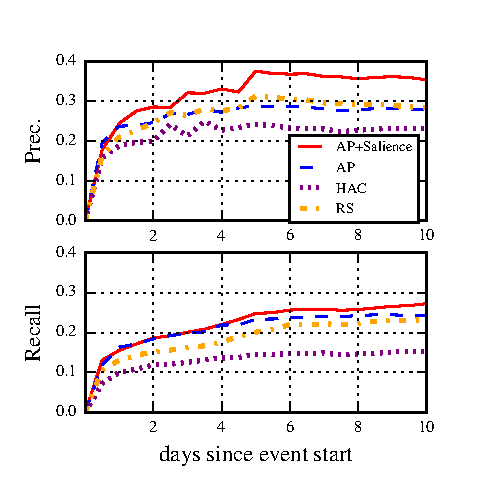
\includegraphics[]{chapter3/figures/rouge-time.eps}
\caption{System ROUGE-1 performance over time.}
\label{fig:3_aps_rouge_time}
\end{wrapfigure}


    \subsubsection{Results}

\autoref{tab:aps_rouge}  shows  our  results  for  system  output
samples against the full summary of nuggets using \textsc{Rouge}. 
This improvement is statistically significant  for  all  ngram  
precision,  recall,  and  F-measures at the
$\alpha=.01$
level using the Wilcoxon
signed-rank test.
\textsc{AP+Salience}
maintains    its    performance
above  the  baselines  over  time  as  well.
\autoref{fig:3_aps_rouge_time}  shows  the  \textsc{Rouge-1}  scores  over  
time.
We  show  the  difference  in  unigram  precision
(bigram  precision  is  not  shown  but  it  follows a
similar  curve).
Within  the  initial  days  of  the
event,  \textsc{AP+Salience}
is  able  to  take  the  lead
over  the  over  systems  in  ngram  precision.   The
\textsc{AP+Salience}
model is better able to find salient
updates earlier on; for the disaster domain, this is
an especially important quality of the model.
Moreover, the \textsc{AP+Salience} recall is not diminished by the high 
precision and remains competitive with \textsc{AP}. 
Over time \textsc{AP+Salience}'s recall also begins to pull away, 
while the other models start to suffer from topic drift.


\autoref{fig:3_aps_autots} shows the Expected Gain and Comprehensiveness 
across a range
of  similarity  thresholds,  where  thresholds  closer
o 1 are more conservative estimates. The ranking
of the systems remains constant across the sweep
with \textsc{AP+Salience}
beating all baseline systems.
Predicting salience in general is helpful for keeping a summary on topic as the  \textsc{RS}  approach out
performs  the  clustering  only  approaches  on  expected gain.
When looking at the comprehensiveness of the
summaries \textsc{AP} outperforms \textsc{AP+Salience}.  
The compromise  encoded  in  the  \textsc{AP+Salience}
objective function, between being representative and
being salient, is seen clearly here where the per-
formance of the \textsc{AP+Salience}
methods is lower
bounded by the salience focused  RS  system and
upper bounded by the clustering only AP system.
Overall, \textsc{AP+Salience}
achieves the best balance
of these two metrics.

\begin{wrapfigure}{R}{0.45\textwidth}
    \center
  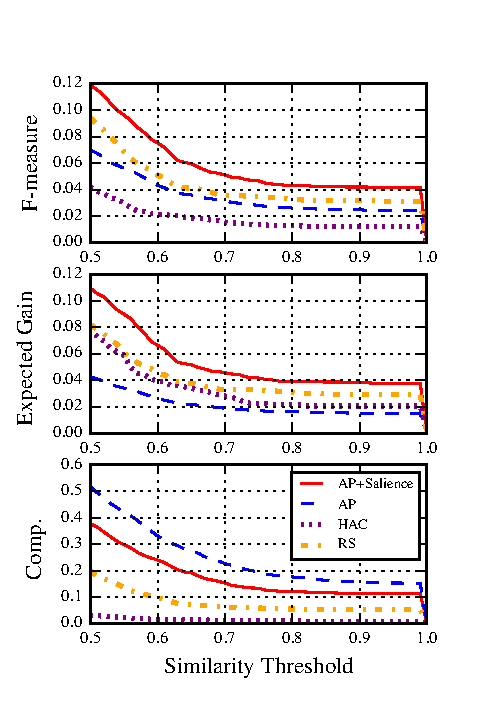
\includegraphics[]{chapter3/figures/nuggets-metrics2.eps}
\caption{Expected Gain and Comprehensiveness performance.}
\label{fig:3_aps_autots}
\end{wrapfigure}


